\documentclass[a4paper]{article}


\usepackage[english]{babel}
\usepackage[utf8x]{inputenc}
\usepackage{multirow}
\usepackage{hhline}
\usepackage{graphicx}
\usepackage{subfigure}
\usepackage[colorinlistoftodos]{todonotes}
\usepackage{fancyhdr}
\usepackage{amsmath}
\usepackage{tabularx}
\usepackage{url}
\usepackage[encapsulated]{CJK}
%\usepackage{fontspec}
\usepackage{caption}
\usepackage{indentfirst} 
\usepackage{float}
\usepackage{amsmath}
\captionsetup[table]{skip=0pt}


%\setmainfont{Microsoft YaHei UI}

\begin{document}
\begin{CJK*}{UTF8}{gkai}

\title{
\begin{figure}[!h]
\centering
%\includegraphics[width=0.9\textwidth]{logo.png}
\end{figure}
\vspace{5mm}
\textbf{Interactive Relighting of Dynamic Refractive Objects}
\text{Implementation Specification}
\vspace{7mm}
\date{}
}


\author{
  应哲敏\\
  \texttt{3120101966}\\
  \texttt{Computer Science}\\
  \texttt{yingzhemin@hotmail.com}
  \and
  巩炳辰\\
  \texttt{3120000140}\\
  \texttt{Computer Science}\\
  \texttt{gbc@zju.edu.cn}
}


\maketitle
\vfill
\begin{center}
June 2015
\end{center}

\newpage


\pagestyle{fancy}
\lhead{}
\rhead{Page \thepage{} of \pageref{page:EndofDoc}}


\begin{abstract}
In this documentation we just specify how we implemented the relighting of dynamic refractive objects as described by Sun, X. et al.[2008].\cite{citation:paper} All credits go to the authors of the paper. Thanks to thier working.


As the fancy paper was published in 2008, situations have changed a lot. We altered some methods used in the original pipeline. So in our implementation, more workload is done on GPU, which results in a more coherent pipeline. 
\end{abstract}


\section{Introduction}
\subsection{Original pipeline}
We briefly describe the original pipeline here, for the convenience of describing our implemented pipeline. The complete original pipeline is depicted in Figure \ref{fig:pipeline}.

\begin{figure}[H]
\centering
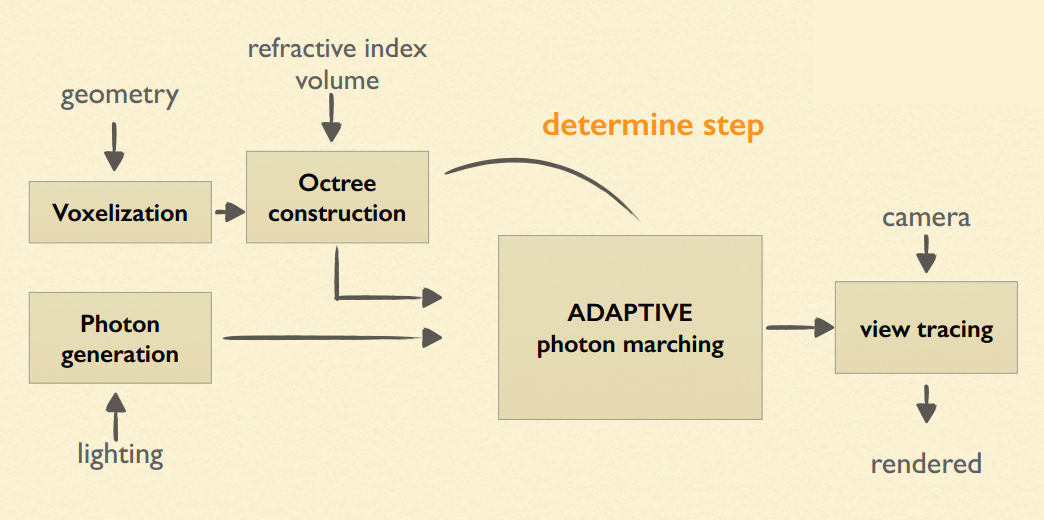
\includegraphics[width=0.9\textwidth]{pipeline.png}
\caption{\label{fig:pipeline}Original pipeline}
\end{figure}


\begin{enumerate}
\item Voxelization

Converts triangle-mesh surfaces into volumetric data. As the pipeline traces photon path inside the mesh, a voxel-based representation of the index of refraction \textit{n}, the scattering coefficient $\sigma$, and the extinction coefficient $\kappa$ is required.

\item Octree construction

Analyzes the index of refraction data and produces an octree describing the regions of space in which the refractive index is nearly constant.

\item Photon generation

Generates photons with initial positions and diretions, which will traverse the scene later. 

\item Adptive photon marching

Advances each photon along its path through the scene. Step length is chosen adaptively using the formerly constructed octree.

\item Radiance storage

Deposits radiance into all the voxels that each photon traverses.

\item Viewing pass

Renders an image by tracing viewing rays from the camera into the scene and calculating the amount of radiance that reaches the camera along each ray.

\end{enumerate}


\subsection{Technical details}
All the data used in this documentation are obtained in an environment as follows.
\begin{itemize}
\item Model: Stanford Bunny with 5002 faces and 2503 vertices.
\item Rendered resolution: 1024x576
\item Voxelization resolution: 128x128x128
\item Generated photons: 20000 - 70000
\item GPU card: NVIDIA GT 750M
\item Development kits: Visual Studio 2013, OpenGL 4.3, CUDA 7.0
\item Operating system: Microsoft windows 8.1 Pro 64 bit
\end{itemize}


\section{Our Implementation}
\subsection{Voxelization}
\subsubsection{Voxelpipe}

In the original pipeline, voxelization is accomplished by rendering the mesh in a sliced schema. We tried this method,  but failed to do this fast enough. 

We aimed to accomplish the voxelization in less than 100 ms. Suppose we have 100 ms, then for a voxelization procedure with resolution 128x128x128, we have to render this mesh in an extremely high frame rate up to 1280 fps, without other processing. In our experiment, we achieved to render a planar 500x500 picture at 400-500 fps. And moreover, we do not have a GPU rasterizer, we have to rely on the rendering pipeline of OpenGL and this requires additional interoperation between OpenGL and CUDA, which slows down the voxelization a bit more.

So we turned to other voxelization methods. We found a seemingly powerful tool on NVIDIA Reseach website which claims to be programmable. Roughly speaking, this method finds all voxels overlapped by each triangle on the mesh surface and then leverages the fast radix sorting on GPU to get the voxelized mesh. The details of this 3D voxelization method is described by Jacopo Pantaleoni [2011].\cite{citation:voxelpipe} We obtained the source code via Google Code. Unfortunately, the author ceased maintenance in 2011, when the version of CUDA was 4.x. We have to modify and adapt the codes to newer version of CUDA.\footnote{Related code: FILE: src/voxelization.cu, LINE: 386-701}

\subsubsection[Voxel hull filling]{Voxel hull filling\footnote{Related code: FILE: src/voxelization.cu, LINE: 192-234}}
What was more unfortunate, Voxelpipe only gave us a hollow voxelized surface, but not a solid one. So we decided to fill the mesh. We tried scanline and path finding, both resulted in unsatisfying outcomes. Finally, we devised a diffusion simulation based filling algorithm. 

We require the user to choose one internal point of the mesh, like the paint bucket tool in image editing softwares. Alternatively we can design algorithms to find one voxel , which is much more easier then finding all, and frees the users from the choosing operation. We label the chosen internal one by 2, and the formerly obtained voxels by 1, and in the meanwhile, others by 0. In every loop, a 0-labeled voxel looks into the 26 neighbours near it. If it finds at least one 2-labeled neighbour, it labels itself by 2 and exit the loop. Not soon, all internal voxels will be labeled by 2. This procedure is depicted in Figure \ref{fig:onewatch} and \ref{fig:fill}.

\begin{figure}[H]
\centering
\subfigure[Choosing and labeling]{
\label{fig:onewatch}
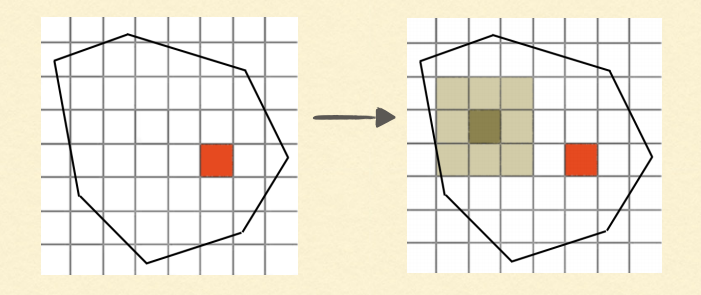
\includegraphics[width=0.5\textwidth]{onewatch.png}}
\hspace{0in}
\subfigure[Filled voxels]{
\label{fig:fill}
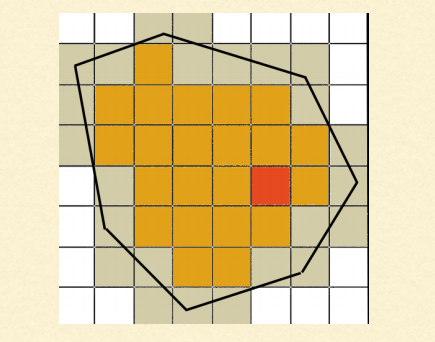
\includegraphics[width=0.3\textwidth]{fill.png}}
\caption{Filling}
\label{fig:subfig} 
\end{figure}


In this algorithm, one vital problem is leaking (Figure \ref{fig:leaking}). We solved this problem by using a 26-separating voxelization (Figure \ref{fig:26sep}). And note that, this algorithm exits when the total 2-labeled voxels stops to increase or the loop number reaches a top bounding limit (the half dimension of the voxelized mesh, $\frac{128}{2}$ in this case).


\begin{figure}[H]
\centering
\subfigure[Leaking]{
\label{fig:leaking}
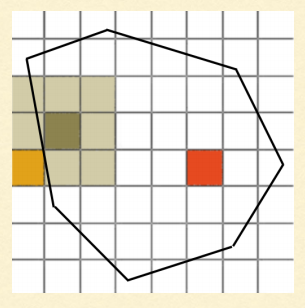
\includegraphics[width=0.4\textwidth]{leak.png}}
\hspace{0in}
\subfigure[26-separating]{
\label{fig:26sep}
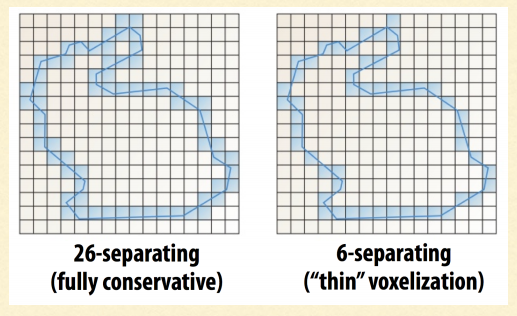
\includegraphics[width=0.5\textwidth]{26sep.png}}
\caption{Leaking and solution}
\label{fig:subfig} 
\end{figure}

In fact, this algorithm takes $O(n^4)$ time on CPU, but thanks to the warp based threads scheduling feature of CUDA library, one voxel does not stay in an invalid loop for long. We found the filling takes only $\frac{1}{3}$ time of the voxelization time and converges pretty early. The performace is shown in Figure \ref{fig:fillperformance} in \textit{ms} unit.

\begin{figure}[H]
\centering
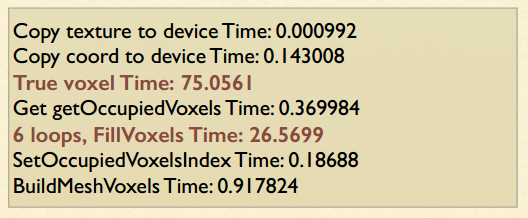
\includegraphics[width=0.7\textwidth]{fillperformance.png}
\caption{\label{fig:fillperformance}Filling performance}
\end{figure}


\subsubsection{Smooth index of refraction}
In the original pipeline, to get smooth variation near the surface of the mesh, it adopts a rather complex super-sampling and down-sampling procedure. We noted that there must be one input into the pipeline. So we did not store the index of refraction in the voxels. In stead, we referd to the original input in later stages in the pipeline. After all, the original input is the most precise one we can get. 

And also, we used a so called \textit{refraction map}(Figure \ref{fig:reframap}) in our early development and later we adopted analytic expressions. We found analytic expression is flexible enough to get the desired refraction distribution. And two of its overwhelming advantages are: it is perfectly precise; it is easy and fast to calculate the gradient.

\begin{figure}[H]
\centering

\includegraphics[width=0.4\textwidth]{reframap.png}
\caption{\label{fig:reframap}Refraction map}
\end{figure}


\subsection[Octree construction]{Octree construction\footnote{Related code: FILE: src/photon\_inline.h, LINE: 143-396}}
Our implementation of the octree is totaly the same as the paper describes. What need to be specified is the data storage, since other implementation details are straightforward. The octree is stored in linear layout in the VRAM. This allows us to access any node on any level according to several easily deduced equations. And the numbers are almost all exponentials of 2, which allows us to optimize the codes using bit operations.

Some equations and implementations are as follows.

$$\mbox{total\_size} = \frac{1}{7} {(2^{3*logN+3}-1)}$$
\begin{figure}[H]
\centering
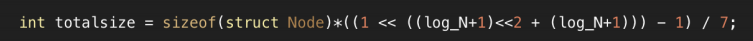
\includegraphics[width=0.9\textwidth]{eq1.png}
\end{figure}

$$\mbox{grid\_on\_level\_n} = 2^{3*(logN-n)}$$
\begin{figure}[H]
\centering

\includegraphics[width=0.9\textwidth]{eq2.png}
\end{figure}

$$\mbox{offset\_level\_n} = \frac{1}{7}(2^{3*(logN+1)} - 2^{3*(logN-n+1)})$$
\begin{figure}[H]
\centering
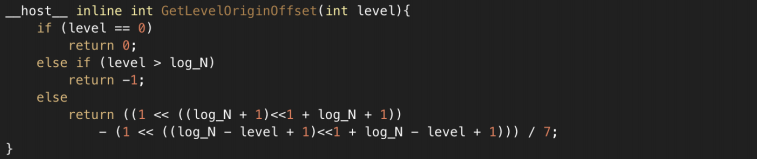
\includegraphics[width=0.9\textwidth]{eq3.png}
\end{figure}

\begin{eqnarray*}
\mbox{In level n, a voxel with offset \textit{offset}:} \\
dim & = & 2^{N-level} \\
x & = & \frac{{offset}}{ dim^2}\%dim \\
y & = & \frac{{offset}}{ dim}\%dim \\
z & = & {offset}\%dim \\
\mbox{level\_origin} & = & 8 * x *dim^2 + 4 * y *dim+ 2 * z
\end{eqnarray*}
\begin{figure}[H]
\centering
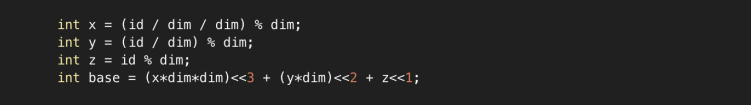
\includegraphics[width=0.9\textwidth]{eq4.png}
\end{figure}


\subsection[Photon generation]{Photon generation\footnote{Related code: FILE: src/photon\_inline.h, LINE: 1242-1406}}
As the paper proposes, photon generation is much similar to shadow map.

We set up an additional frambuffer in OpenGL with color buffer and depth buffer. The camera is put at the exact position of the light, and only the mesh is drawn. As we enabled the depth test, only the faces directly seen by the light will be drawn in the final framebuffer. Here, the small trick is we kept the world coordinates of each drawn vertex in the vertex shader and passed it to the fragment shader. In fragment shader, we used the three RGB channels of color to store the XYZ coordinates. The related GLSL program and the resulted texture are as Figure \ref{fig:depthshader} and Figure \ref{fig:depthcolor} show.

\begin{figure}[H]
\centering
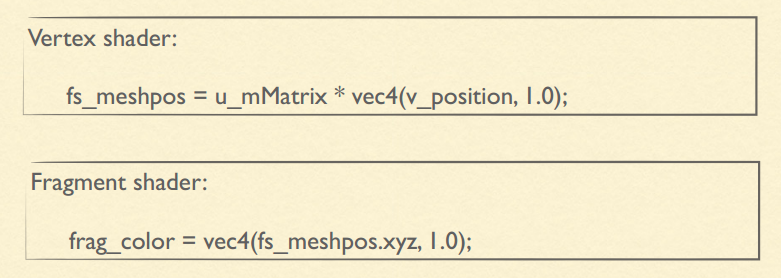
\includegraphics[width=0.7\textwidth]{depthshader.png}
\caption{\label{fig:depthshader}Shaders in photon generation}
\end{figure}


\begin{figure}[H]
\centering
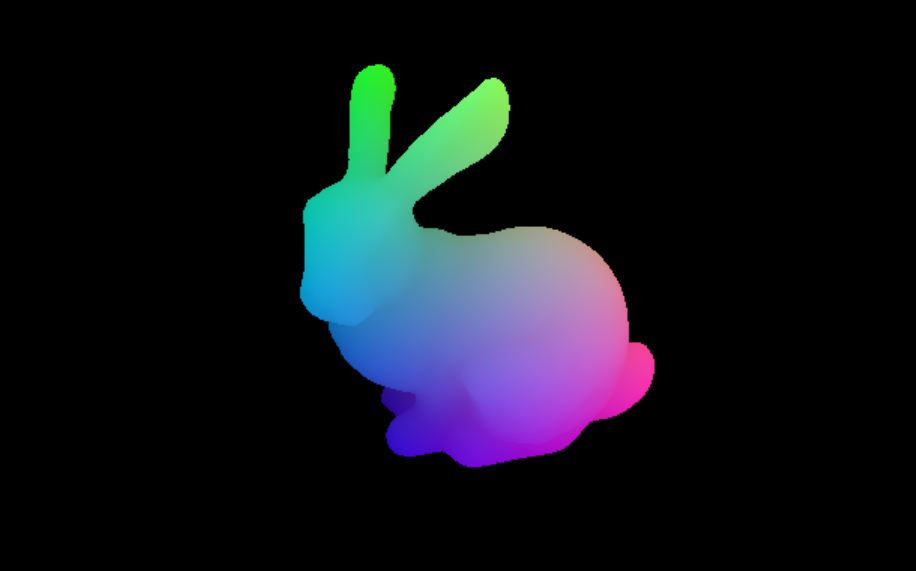
\includegraphics[width=0.7\textwidth]{depthcolor.png}
\caption{\label{fig:depthcolor}Rendered texture with world coordinates}
\end{figure}

World coordinate to color texture rendering is done by OpenGL and later the texture is scanned to generate the photon list. To reduce the number of photons generated, the photons that may not traverse the mesh should be discarded. We only count the colored pixels. When scanning, pixels may be interpolated to produce more photons if the total amount is small or may be down sampled to cut down the total amount if the photons are too many. Together with the position and radiance of the light, we can get the final photon information list with initial position, direction and radiance.

\subsection{Adptive photon marching}
\subsubsection[Photon march]{Photon march\footnote{Related code: FILE: src/photon\_inline.h, LINE: 920-946}}
To march the photons, we followed the ray equation of geometric optics.

\begin{eqnarray*}
x_{i+1} & = & x_i + \frac{\Delta s}{n} v_i \\
v_{i+1} & = & v_i + \nabla s \Delta n
\end{eqnarray*}

These equations are straightforward and can be easily turned into codes.

\subsubsection[Step determination]{Step determination\footnote{Related code: FILE: src/photon\_inline.h, LINE: 602-700}}
When determine the step length in photon marching, we encountered some problems to do with the choice between discrete and continuous. To take advantage of the octree, one may let the step length be one or several times of the voxel size. But the direction is hard to determine. If the direction is continuous, then due to discrete float number rounding, the direction varies in a jumping form. And if the direction is discrete, we can use only 26 directions. Both these two situations result in unsmooth results in our experiment.

So we adopted a continuous way for both the step length and the direction. We still leveraged the constructed octree, but only to obtain the largest size of the region in which the index of refraction is almost constant. Then in this region, we calculated the intersection point on one of the region surface with the photon marching ray. Given the direction, one ray can only intersect with three surfaces of the cube, so we used an enumerating calculation as follows.

for: known\_index = 0 : 2
\begin{multline*}
{pos\_next_{known\_index}} = {origin}_{known\_index} \\
+ Sign({direction}_{known\_index} +1)*{region\_size}*\frac{1}{2} 
\end{multline*}

for: not\_known\_index = (known\_index + i)\%3, i = 1, 2

\begin{multline*}
$${pos\_next}_{not\_known\_index} = \frac{{pos\_next}_{known\_index} - {pos}_{known\_index}}{{direction}_{known\_index}} \\
* {direction}_{not\_known\_index}  \\
+ {pos}_{not\_known\_index}$$
\end{multline*}

We was anxious about the intersection calculation taking long time. But it turned out to be fast. In one test, it measured 283,366 ns, as opposed to the calculation of the index of refraction which took 174,550 ns.

After the calculation of intersection, we used the length of position-intersection vector as marching step length. But this is not the final. This length is compared with the user provided step lower or upper limit and a default lower limit(one voxel). Finally, we multiplied the length with about 1.1 to push the photon a bit further out of the current region.


\subsubsection[Rasterization and radiance storage]{Rasterization and radiance storage\footnote{Related code: FILE: src/photon\_inline.h, LINE: 762-901}}
The original pipeline adopts a rather complex workaround here, due to the unavailability of atomic operations in CUDA and disability to rasterize 3D texture in OpenGL. After refering to the documentations of CUDA, we noticed that GPU of compute capability 2.x or above does have an atomic operation on float numbers.

So we wrote our line rasterizer. The rasterizer is quite naive but is adequate to the line segmentation task. We found the main direction of the line, along which the line goes through most voxels. Then we step through the voxels along this direction, storing values in each traversed voxel.



\subsection{Viewing pass}
Viewing pass is much similar to adaptive photon marching. The difference is the camera is set at the position of eyes and step length is not adaptive but fixed. Some other implementation details are in the following sections.

\subsubsection[Resulted textures]{Resulted textures\footnote{Related code: FILE: src/photon\_inline.h, LINE: 1409-1468}}
As CUDA can not directly render the results on the display, we have to store the results in several textures and transfer them to OpenGL. We used four textures: color texture for environment map, radiance texture for environment map, color texture for traced view ray and radiance texture for traced view ray. Except the first one, the other three are copied from CUDA to OpenGL to display. Texture mixup is done in fragment shader because in this way we can omit lots of pixels that do not come from the textures.

The reason we distinguished color and radiance is that human eyes are more sensitive to luminance information. So we can take more control on the luminance information by seperating it from color. Another reason is that radiance results must be normalized according to the amount of photons, but the color results need not.

In the fragment shader, Gaussian blur is applied to make the results more smooth.

\subsubsection[Single scattering]{Single scattering\footnote{Related code: FILE: src/photon\_inline.h, LINE: 883-901}}
We treated the single scattering inside mesh and in air as Mie Scattering. The intensity of scattered light is calculated as proportional to viewing angle cosine value.

$$I(\theta)=I_i(1+cos^2{\theta})$$

\subsubsection{Color mixing}
Color mixing includes two aspects. One is mixing two colors, and another one is mixing color with luminance.

Colored light goes through one transparent object and then through another transparent object, what is the resulted color of the light? This problem is actually hard to solve. We first refered to a dedicated paper on this topic, but later found it is too complex.\cite{citation:color} Our second trial was the subtractive color system CMYK, and found the performance suffered. So at last, we just took the minimum of every RGB channel. This is coarse treatment but the result is acceptable.

Color and luminance mixing is more systematic.  We converted the RGB value to HSL color space. In HSL color space there is a luminance channel and we just increased or decreased the L channel by some degree. The color is converted back to RGB color space for display. Color and luminance mixing is done in fragment shader.\footnote{Related code: FILE: src/shaders/default.frag, LINE: 57-166}



\subsection{Optimization}
To improve the frame rate and provide a more smooth interaction, we spent much time on optimization. Two main techniques are using local memory more and making less function call.

\subsubsection{Local memory and global memory}
If we transfer data from CPU to GPU using \textit{cudaMemcpy} or allocate memory using \textit{cudaMalloc}, the related memory resides in global memory. For every thread, it has its own local memory and local registers. Copy the data from global memory first and operate on the data locally and then copy the data back to global memory, this is much faster than operaing on the global memory directly. Operation and performance differences can be seen in Figure \ref{fig:gandl} and in Figure \ref{fig:gandlperf} (unit is ns). We see the performance is nearly doubled.


\begin{figure}[H]
\centering
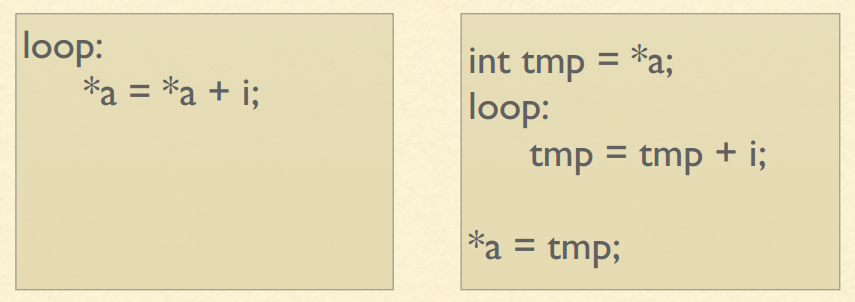
\includegraphics[width=0.5\textwidth]{gandl.png}
\caption{\label{fig:gandl}Operate globally and locally}
\end{figure}


\begin{figure}[H]
\centering
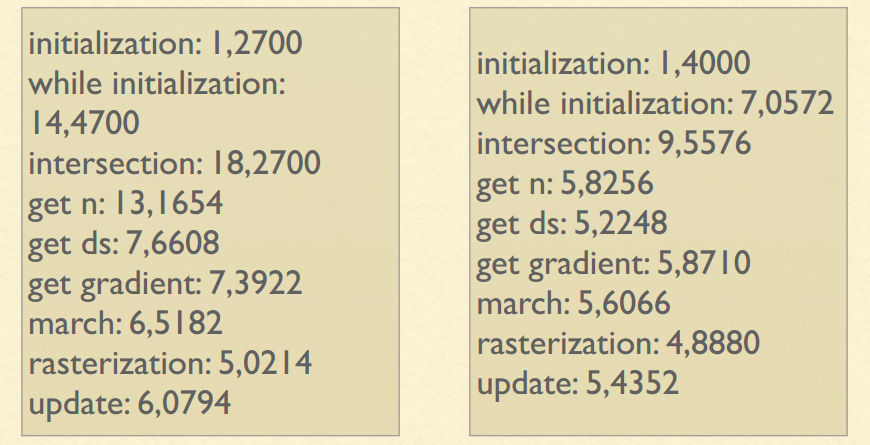
\includegraphics[width=0.5\textwidth]{gandlperf.png}
\caption{\label{fig:gandlperf}Preformance difference between two kinds of operation patterns (ns)}
\end{figure}

\subsubsection{Make less function call on device}
We found function calls on device are expensive. Even the function is inlined, it seems that the compile forgets the \textit{inline} keyword. A small experiment is as Figure \ref{fig:funccall} shows.

\begin{figure}[H]
\centering
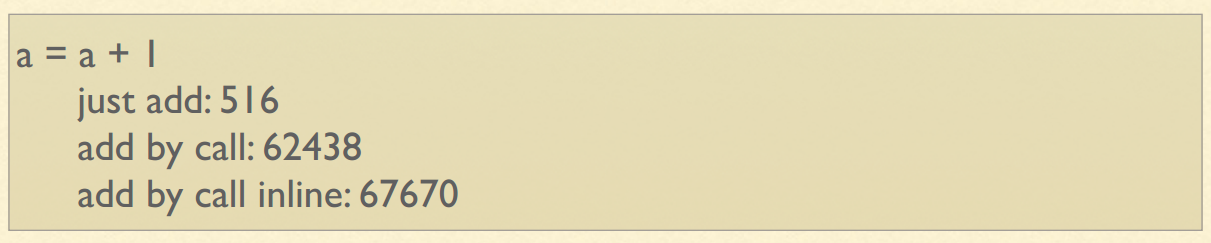
\includegraphics[width=0.7\textwidth]{funccall.png}
\caption{\label{fig:funccall}Preformance difference between three kinds of Add operation patterns (ns)}
\end{figure}

So we replaced all function definitions on device with macro definitions. This optimization cut down $\frac{1}{3}$ time.


\section{Results}
Here we present some screenshots of the rendered results.

The Stanford bunny:
\begin{figure}[H]
\centering
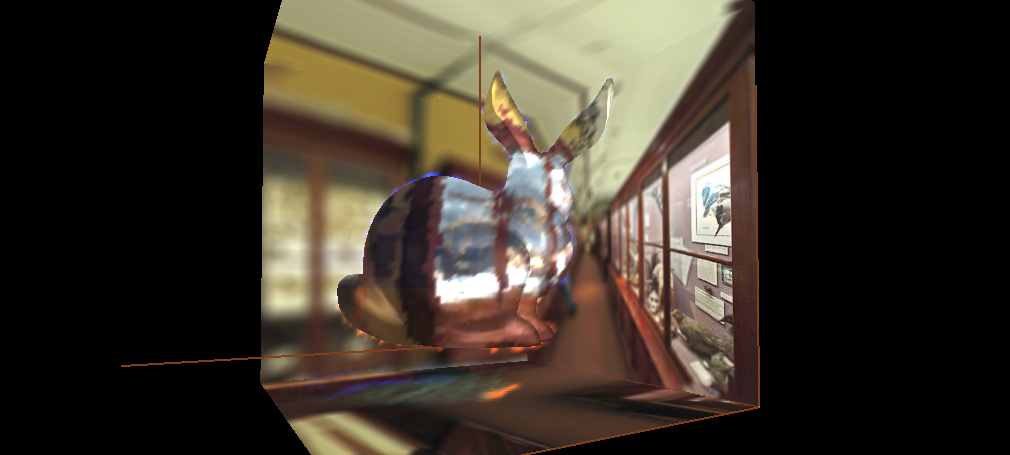
\includegraphics[width=0.7\textwidth]{bunnyres.png}
\caption{\label{fig:bunnyres}}
\end{figure}

Two balls:
\begin{figure}[H]
\centering
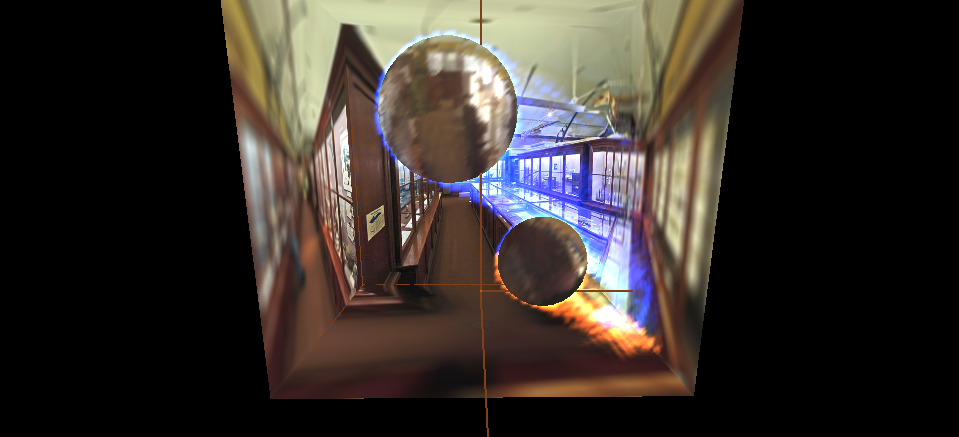
\includegraphics[width=0.7\textwidth]{ball1.png}
\caption{\label{fig:ball1}}
\end{figure}



\begin{figure}[H]
\centering
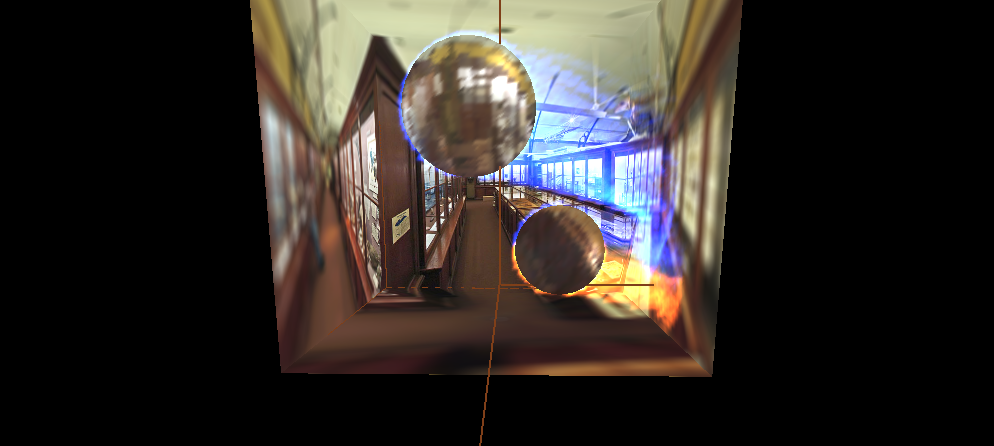
\includegraphics[width=0.9\textwidth]{ball2.png}
\caption{\label{fig:ball2}}
\end{figure}

\begin{figure}[H]
\centering
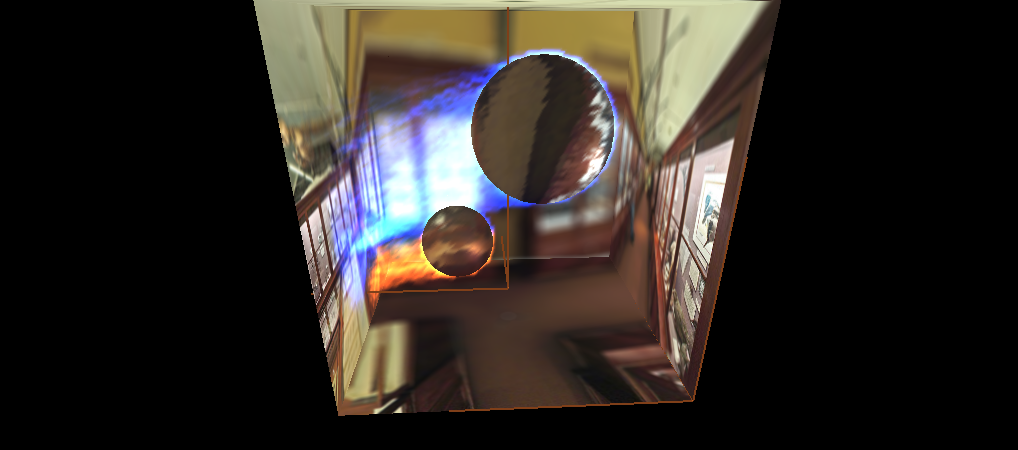
\includegraphics[width=0.9\textwidth]{ball3.png}
\caption{\label{fig:ball3}}
\end{figure}

\begin{figure}[H]
\centering
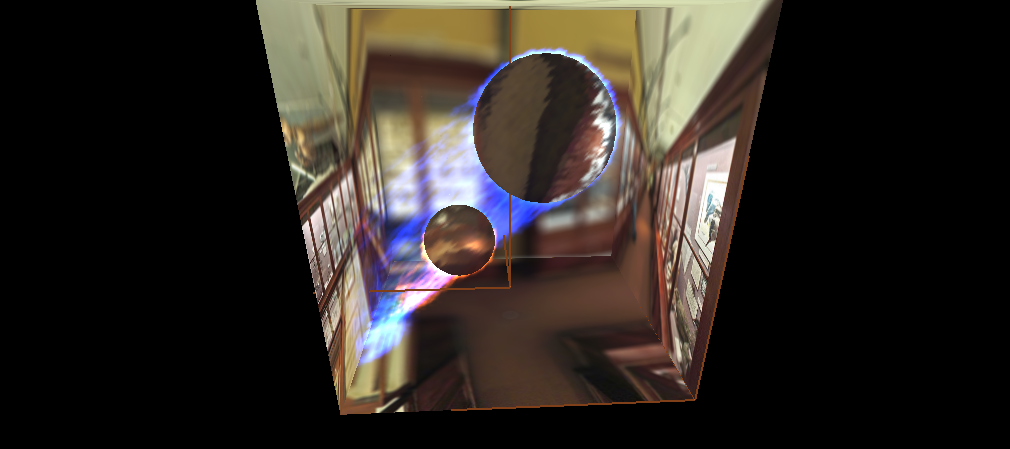
\includegraphics[width=0.9\textwidth]{ball4.png}
\caption{\label{fig:ball4}}
\end{figure}

\begin{figure}[H]
\centering
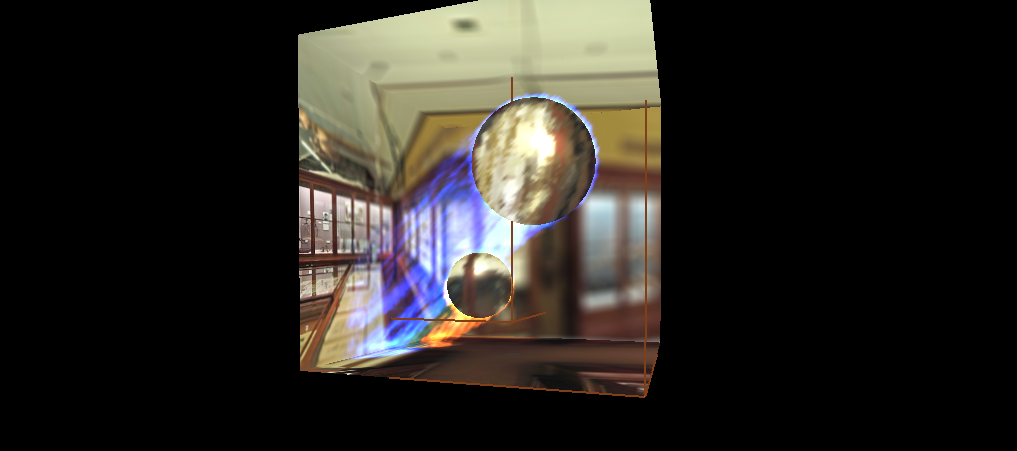
\includegraphics[width=0.9\textwidth]{ball5.png}
\caption{\label{fig:ball5}}
\end{figure}


Unfortunately, our visual results are not as good as the paper presents.

The frame rate is about 8-12 fps on the machine specified formerly. As the equipments are much different from those used by the authors of the paper, it is meaningless to compare performance results.

\section{Conclusion}
In our implementation, only photon generation and rendering is done by OpenGL. Others are done by CUDA. This reduces data transfer dramatically.

Though we implemented the whole pipeline, our rendered result is not so satistying visually. We think much working need to be done to improve the visual results.

\end{CJK*}


\bibliography{bib} 
\bibliographystyle{ieeetr}

\label{page:EndofDoc}
\end{document}


